\section{Simulation tool development}

\subsection{The importance of simulation tools}

\noindent AM-based L1 tracking is a relatively complex task requiring a precise modelization before going to hardware implementation. This modelization is done via a dedicated simulation framework comprising:

\begin{itemize}
\item The model of the new tracker geometry implemented within the official CMS software chain (CMSSW)
\item The definition of the trigger tower
\item The definition and the production of the pattern banks for each trigger tower
\item The emulation of the AM-based pattern recognition within CMSSW
\item A set of track fitting procedures compatible with an FPGA implementation, coded within CMSSW
\end{itemize}

\noindent The following sections of this part are providing a description of the different steps necessary to setup this modelization. 

\subsection{Tracker geometry and trigger tower definition}

\noindent The geometry description and the trigger sector definition is provided by a standalone program: the TkLayout tool~\cite{bib:TkLayout}. For the geometry, this tool builds the xml files necessary to the CMSSW simulation stage. Then, using rates obtained from simulation and L1 tracking trigger requirements (in particular the minimal $p_T$ required for the tracks), the TkLayout tool can be used to optimize the trigger towers definitions. The goal here is to define the largest possible towers with a reasonable input data rate per layer, and to minimize the data sharing between towers. After performing this task, the TkLayout tool provides a simple text file containing, for each sector, a list of the tracker modules belonging to that sector. This file defines the structure of the track trigger system, and is hence is the basis of the L1 tracking stage.
  
\subsection{Pattern bank generation}

\noindent Bank generation is done via a dedicated standalone C++ program~\cite{bib:AMEmulator}. The main bank generation procedure is sketched on Fig.~\ref{fig:BkGen}. In order to produce a bank, two inputs are needed: a large simulated sample of single particle gun events (traditionally muons) covering the whole L1 track trigger acceptance requirements, and the TkLayout file providing the trigger towers definition.

\begin{figure}[ht!]
\centering
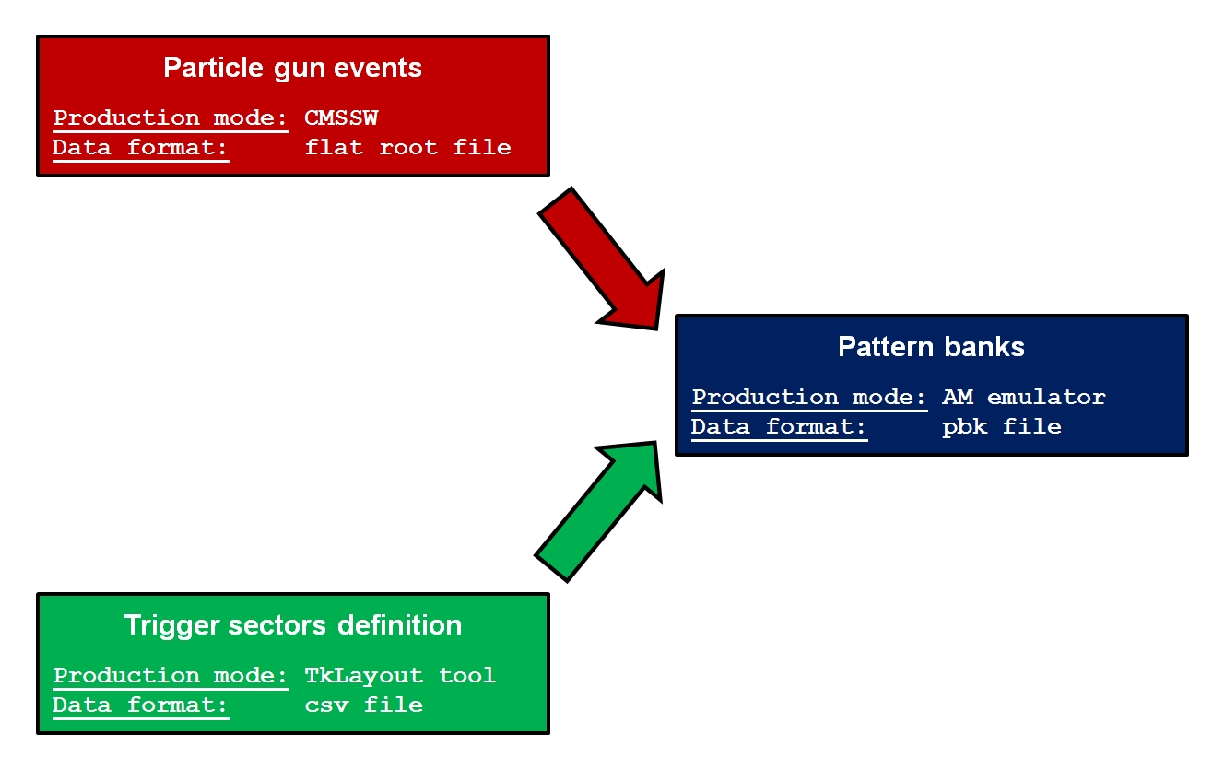
\includegraphics[width=0.6\columnwidth]{Plots/BankGen.eps}
\caption{Pattern bank generation principle}
\label{fig:BkGen}
\end{figure}

\noindent Based on these inputs, the code is able to produce a pattern bank for any trigger tower. Bank parameters can be set in the configuration file of the generation job. A complete description of the available option is provided in~\cite{bib:AMEmulator}.  

\noindent The bank generation algorithm, as it is implemented in the emulator, is summarized on Fig.~\ref{fig:BkGenDet}.

\begin{figure}[ht!]
\centering
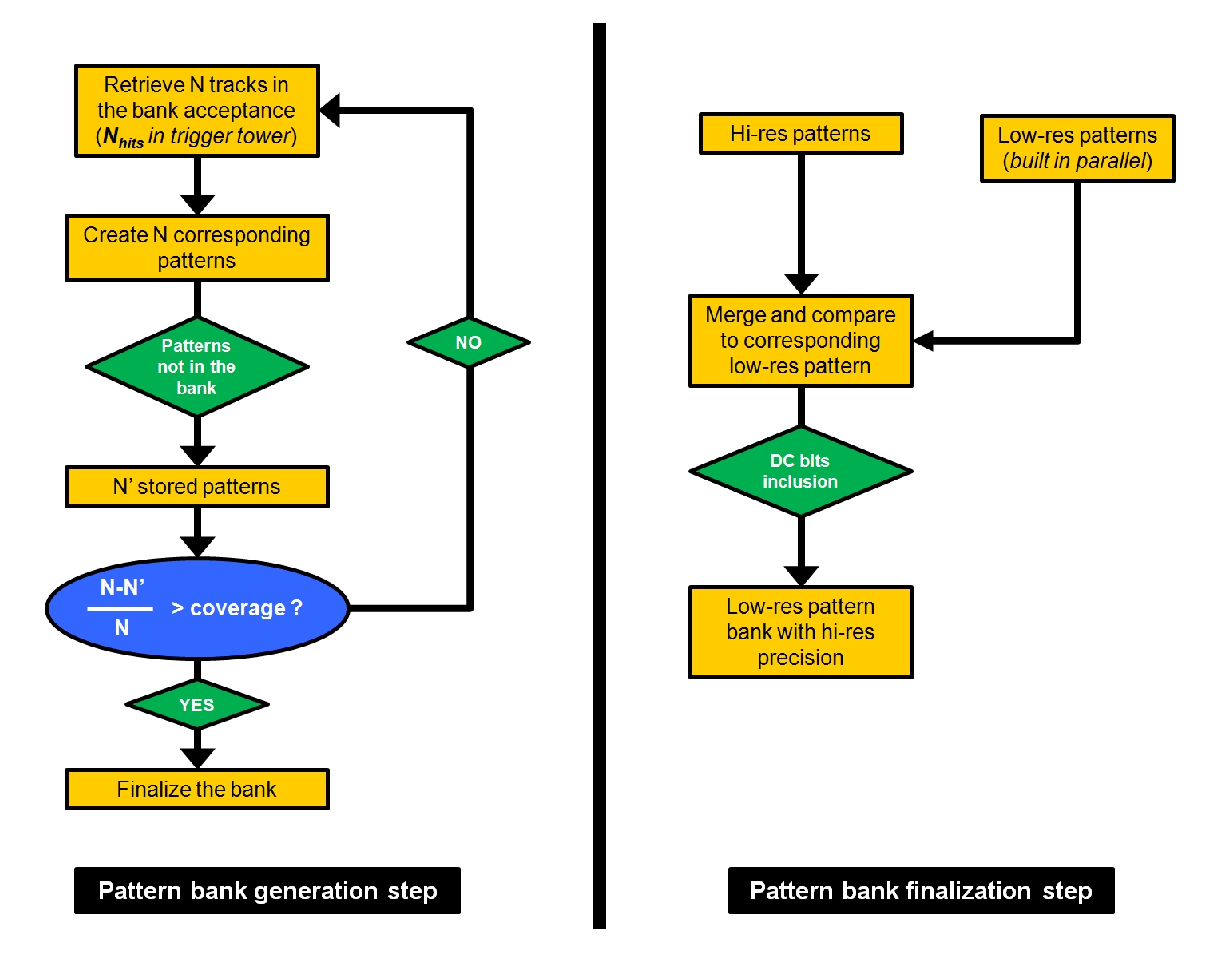
\includegraphics[width=0.6\columnwidth]{Plots/BankGenDetail.eps}
\caption{Pattern bank generation workflow: from track sample to pattern bank}
\label{fig:BkGenDet}
\end{figure}

\noindent This algorithm can be divided into two steps: bank production and bank finalization. As shown on the left diagram, the bank production is performed iteratively. An iteration starts by the collection of a set of $N$ tracks satisfying the pattern bank acceptance requirements in the input data sample (in our case $N=40000$). This acceptance requirement is defined by the parameter $N_{hits}$, which corresponds to the number of different layer/disks in which the particle has induced stubs in the trigger tower considered\footnote{This number should not be confused with the total number of stubs induced by the particle. If a track induces two stubs in a given layer (for example in an overlap area), these stubs will just count as one in $N_{hits}$.}.

\noindent A track can be used to produce a pattern only if its $N_{hits}$ value is equal to the pattern size set in the job configuration. Of course the pattern made from the track is stored in the bank only if not already in. Iteration ends when $N$ tracks have been collected. At this point, the proportion of tracks collected which were leading to an already stored pattern is computed. If this proportion, defined as the bank coverage, is larger than the coverage initially required, the iteration stage stops.

\noindent Once the required coverage has been reached, the bank is finalized. The procedure is described in the right part of Fig.~\ref{fig:BkGenDet}. At this point, it's not one, but two banks which have been built. Indeed, each new pattern is automatically linked to a low-resolution mother pattern. The resolution of this mother pattern is direclty related to the number of DC bits. The width of the low-res patterns is indeed $2^{N_{DC}}$ larger than the width of the high-res ones. For example, if one requires 2 DC bits, and built pattern with a superstrip size of 32 strips, the width of the low resolution patterns will be 128 strips. 

\noindent The low-res bank building follows the same procedure than the hi-res bank. But in addition, each low-res patterns is linked to a set of hi-res patterns. Before storing the low-res pattern in the banks, hi-res patterns belonging to it are merged. The merging result is then compared to the low-res pattern, and the hi-res granularity is kept whenever possible. On the other hand, if all the super-strips are used in a given layer, corresponding DC bits are applied.

\noindent Using this procedure provides the possibility to get high-resolution precision for the price of a low resolution bank. 


\subsection{Pattern recognition}

\subsubsection{Software principle}

\noindent The pattern recognition is done using the same code than the bank generation. This code has been interfaced with the CMS software framework (CMSSW). It uses the official CMSSW stubs and stores the patterns as official CMSSW track seeds. For debugging purposes, the pattern recognition code can also work standalone, starting from plain rootuple containing the stubs of a given event. 

\noindent The code is working for a given sector. The complete pattern recognition of a given event therefore requires to run in parallel jobs for every trigger tower. The data merging is performed afterwards, so that the final output contains for each event the pattern recognition outcome for all the towers. 


\subsubsection{Estimation of the pattern recognition efficiencies and fake rates}

\noindent The basis of the pattern recognitionefficiency is the number $N$ of matchable tracks. This number is depending on the size of the patterns stored. For patterns made of 6 superstrips, if a missing hit is accepted, any track crossing at least 5 layers in the tower will matchable. 

\noindent The number of layers/disks crossed by the particle within one tower is therefore an important parameter. From now own, it will be mentioned in all the notations. For example, $N_{5}$ corresponds to the number of tracks crossing at least 5 layers/disks in one of the trigger tower.

\noindent Starting from there, the efficiency for a given threshold could be defined as the number of tracks matched in a pattern divided by the total number of tracks: 
\begin{equation}
\epsilon_i = \frac{N^{matched}_i}{N_i}
\end{equation} 

\noindent Then, we define the fake rate as the proportion of patterns which are not containing a good track. 
\begin{equation}
\rho_i = \frac{N^{bad patterns}_{i}}{N^{patterns}_{i}}
\end{equation} 

\noindent This fake rate definition doesn't account for the duplicated patterns. This value is measured by the redundancy,which corresponds to the average number of patterns activated by each good track. The ideal pattern bank for a given threshold $i$ is the one for which $\epsilon_i = 1$ and $\rho_i = 0$.

\noindent Such a bank exists, this is the one for which each possible track in the detector corresponds to one pattern. However, the size of such bank will be prohibitive. On the other side, one could imagine the simplest bank with 1 single pattern defined by the whole detector. Such a bank will have $\epsilon=1$, $\rho = 0$ and $r = 1$, but $\epsilon_{hits}$ will be close to 0. Such a solution would be highly inefficient, as TF would be impossible to process. Therefore the optimal solution lies in between, and one realizes that a parameter will be very important: the size of the patterns. The patterns will have to be sufficiently small in order to get a reasonable $\epsilon_{hits}$, but also sufficiently large in order get a reasonable pattern bank size. 

\noindent Finding the optimal bank is a complex exercise which will be done for the TDR, and hence is beyond the scope of this preparatory note. In this document we present preliminary results obtained using a simple set of pattern banks, which where produced using a large sample of particle gun $\mu^{\pm}$ produced within the following phase space:
\begin{itemize}
\item $0 < \eta_0 < 2.2$.
\item $1.95GeV/c < p_{T_0} < 100GeV/c$, generated randomly in $1/p_T$.
\item $-15cm < z_0 < 15cm$.
 \item $-1mm < d_0 < 1mm$.
\end{itemize}  

\noindent In order to cover correctly the whole $pT$ phase space the sample was divided into three $pT$ ranges: 1.95 to 5 GeV/c, 5 to 20, and 20 to 100. Patterns were made from 32 to 256 strips-wide superstrips (we generate 32 strips banks and used 3 DC bits) in order to get banks of ~1M patterns for each trigger tower. The total number of patterns necessary to cover all the tracker in this configuration is 64~Millions. 

\noindent The following table summarizes the overall efficiencies and fake rates obtained for simple single particles with $p_T>2GeV/c$ using the banks described previously, for $N_{hits}=5$.

\begin{table}[ht!]
\centering
\begin{tabular}{|c|c|c|c|}
  \hline
  Particle type & Muons & Pions & Electrons \\ \hline
  Efficiency ($\epsilon_5$, in \%) &  &  &  \\ \hline
  Fake rate ($\rho_5$, in \%) &  &  &  \\\hline
\end{tabular}
\caption{Stub repartition in the tracker, measured with PU=200 events.}
\label{tad:dev}
\end{table}

\noindent Figures~\ref{fig:PRMU} and {fig:PRELE} shows a summary of the pattern recognition outcome for muons and electrons respectively. The broader turn-on for electrons is mainly due to multiple scattering.

\begin{figure}[ht!]
\begin{minipage}[t]{7.5cm}
\centering
%\includegraphics[width=0.75\textwidth]{Plots/Muon.eps}
\caption{Pattern recognition efficiency for single muons}
\label{fig:PRMU}
\end{minipage}
\hfill
\begin{minipage}[t]{7.5cm}
\centering
%\includegraphics[width=0.75\textwidth]{Plots/AdapSec.eps}
\caption{Pattern recognition efficiency for single electrons}
\label{fig:PRELE}
\end{minipage}
\end{figure} 

\noindent In order to evaluate the fake rate, two types of events were used. Both were overlaid with an average of 140 minimum bias events. In the first set, a single muon was added to minbias contents, whereas in the other sample, a four tops final state was added. This last sample could be considered as a worst case scenario for tracker occupancy, and is therefore particularly useful for studying the maximum rates per modules.   

\noindent The pattern recognition efficiency was also tested, as shown on Fig.~\ref{fig:PR_4tops} for the 4 tops events. As expected, the efficiency is robust against pileup. If a pattern is matched, it will always match independently from the stubs you add around it. What will change is the fake proportion. The fake rates, for both samples are summarized in the following table:

\begin{table}[ht!]
\centering
\begin{tabular}{|c|c|c|c|}
  \hline
  Particle type & Muons & Pions & Electrons \\ \hline
  Efficiency ($\epsilon_5$, in \%) &  &  &  \\ \hline
  Fake rate ($\rho_5$, in \%) &  &  &  \\\hline
\end{tabular}
\caption{}
\label{tad:dev}
\end{table}

\subsubsection{Bank efficiency definition}


\subsection{Further developments and improvements}


\clearpage
